\documentclass[conference]{IEEEtran}
\IEEEoverridecommandlockouts
\usepackage{cite}
\usepackage{amsmath,amssymb,amsfonts}
\usepackage{algorithmic}
\usepackage{graphicx}
\usepackage{textcomp}
\usepackage{hyperref}
\usepackage{xcolor}
\begin{document}
\title{Study on Factors Affecting Country's Growth}

\author{\IEEEauthorblockN{1\textsuperscript{st} Neeraj Gopalakrishnan}
    \IEEEauthorblockA{\textit{Computer Science and Engineering} \\
        \textit{PES University}\\
        Bangalore, India \\
        neerajperso@gmail.com}
    \and
    \IEEEauthorblockN{2\textsuperscript{nd} Hritik Sharma}
    \IEEEauthorblockA{\textit{Computer Science and Engineering} \\
        \textit{PES University}\\
        Bangalore, India \\
        hritiks2012@gmail.com}
    \and
    \IEEEauthorblockN{3\textsuperscript{rd} Priya Gawli}
    \IEEEauthorblockA{\textit{Computer Science and Engineering} \\
        \textit{PES University}\\
        Bangalore, India \\
        priyagawli99@gmail.com}

}

\maketitle
\begin{abstract}
    The goal of this project is to create a basis of analysis that corroborates the relation between factors that affect a country's economy.\\
    In the first stage of this report, we wish to demonstrate the synopsis of the problem statement, explain the data and it's relation using an Exploratory data analysis(EDA]. The problem statement is explored from various angles using other existing papers and kaggle EDAs.\\
    The plan moving further will be to perform a few more EDA/Visualization to further our understand of the dataset and clean to improve the model to be more forgiving and informative for a larger scope of analysis. This will help the model forcast with an even higher accuracy. We also plan to experiment with various models in order to select the most optimal one.
\end{abstract}
\bigskip
\begin{IEEEkeywords}
    Prediction/Forecasting, Macroeconomies, Global Goals(UN's), Multiple Linear regression, Time-Series Analysis
\end{IEEEkeywords}
\section{Introduction}
The economic growth of the country is what defines the countrys development rate in a global scale.
But as the time passes by and the way the goals are aligned to be a more stable economy or the gloabal goal of
being more suststainable has become a primary focus than a higher economic power,
and the means to forecast the growth of the economy becomes more complicated.\\
Almost all of the country's problems can be analysed with the context of its economic growth.

This economic growth has various factors that influence it's trend; some obvious ones like: Gross-Domestic-Procduct(GDP) per Capita, Unemployment rate, Population Growth, Government Expenditure, etc; and some not so obvious ones like: Firms with female ownership, Lending interest rate, etc.
Other than these convential metrics for measuring growth we have:\\
\begin{itemize}
    \item The Impact of Human Resources
    \item Investment of capital
    \item Availability of Natural Resources
    \item Improvement in Technology
\end{itemize}
\bigskip
For our project we will be estimating the GDP on-a-country-basis which will help us project or forecast where the countries GDP might be in the forecoming future.
GDP measures the monetary value of final goods and services—that is, those that are bought by the final user—produced in a country in a given period of time (say a quarter or a year).
It counts all of the output generated within the borders of a country.
GDP is composed of goods and services produced for sale in the country, not only that but also includes some non-market related products sales and it's production, such as defense or education services provided by the government.
An alternative concept, gross national product, or GNP, counts all the output of the residents of a country.
\\
But nowadays since the global goals of UN for countries is to target a sustainable goal development it is necessary for newer alternatives that is subjected to more scrutiny for even the macro factors such as waste produced per capita gained to see if that portion of economic growth is sustainable or not.
\\The goal of our project is to quatify GDP as a factor of growth and be able to estimate how the trends for the future of the economy would be. It focuses more on growth than sustainable development, but we will look into the factors that affect the "Sustainable Development Goals" too
\bigskip
\section{Literature Review}
\emph{A. How big of an impact does expenditure on health care have on GDP?}
\\The study of this research paper attempt to identify an association of the life expectancy with healthcare expenditure and GDP in Bangladesh. The researchers of this study generate the analysis to look for an association of GDP with government funding towards health care sector and life expectancy.
Their study details about the total government spending on heatlth-care as their national expenditure and is calculated as a share of GDP, which can vary according to the country's priorities which it can be contingent on the capacity to pay and fiscal(budgetory) restraints of a fiscal year. Also, the fact that government funding towards healthcare sector is biased based on aspects like distribution of young-older population, urban-to-rural ratios, and burden of contagious and the non-spreading diseases reflects also on the amount of money needed for the healthcare of the country. However, life expectancy is also unequally distributed globally. For example, life expectancy is often better in the developed countries, as compared to that of the developing countries.
\\For the study, they collected total health expenditure and GDP for the year of 1996 to 2006 from “Bangladesh Health Bulletin 2011” and the life expectancy for the same period was taken from “Sample Vital Registration System 2010” respectively. To compare life expectancy with the total health expenditure, fiscal year has been considered. Total health expenditure and GDP were expressed using both the Bangladeshi taka (BDT) and USD [Dollars].
\\Total health expenditure includes all of the payments like spending for doctor's consultation fees, medication, laboratory tests and hospital bills. Here the term life expectancy means an expectation of longevity i.e. expected years for a person to survive. They considered Total Health Expenditure (THE) as dependent variable and independent variables are life expectancy and GDP. They performed the analysis using STATA version 13 SE (College Station, Texas, USA). Graphical presentation and descriptive statistics were performed to present the findings. Multivariate logistic regression was carried out to find the association of total health expenditure with life expectancy and fig1. total health expenditure, GDP and Life expectancy from 1997 to 2007 in Bangladesh. GDP. A conventional cut-off value of 0.05 was taken as statistical significance.
\\From this study, they found a direct relationship of total health expenditure and life expectancy in bi-variable analysis.
\begin{figure}[htbp]
    \centerline{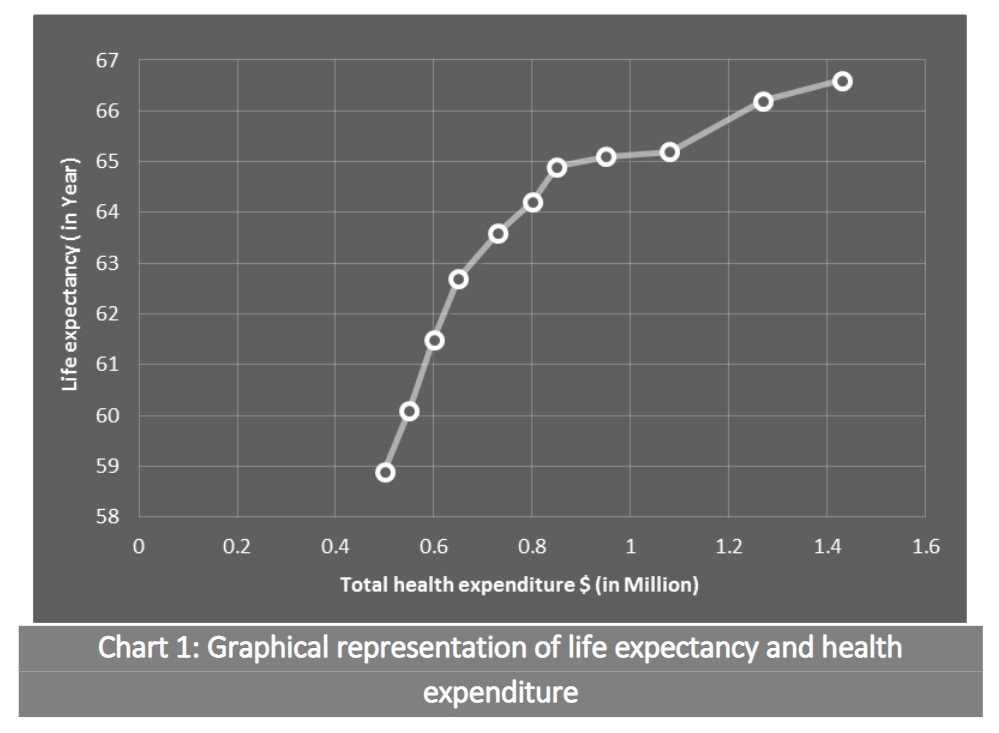
\includegraphics[scale=0.5]{healthcare1.jpg}}
    \caption{Graphical representation of life expectancy and health expenditure}
\end{figure}
\\A priori was considered expecting that both the GDP and LE will have a positive impact on THE. Thus their proposed econometric model is-
\begin{figure}[htbp]
    \centerline{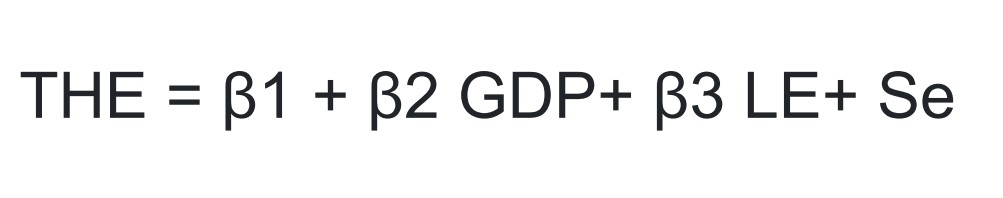
\includegraphics[scale=0.3]{healthcare3.jpg}}
    \caption{Formulae 1.1}
\end{figure}
\\As in Fig.3, Beta1 is the intercept and Se is an error or residual value. This equation has considered Beta2 and Beta3 as the slope for the independent variable of GDP and LE, respectively.
Hence, the results show that total health expenditure is more sensitive to gross domestic product rather than life expectancy of a country. Through further analysis of longitudinal data for different developing countries, the typical association of health expenditure to GDP can be established.
\bigskip

\emph{B. Is there a correlation between power use and economic development, according to empirical research?}
\\The aim of this paper is to examine the empirical co-integration, long- and short-run dynamics, and causal link between Bangladesh's power consumption and real GDP. The analysis demonstrates the short-term unidirectional causal flow between per capita real GDP and per capita electricity consumption. The study's findings also provide compelling evidence of a long-term causal link between per capita real GDP and per capita power usage. And, looks at the existence and direction of a causal link in order to make wise policy choices about the usage of energy. \\
A Granger causality test based on the vector error-correction model (VECM) was used to examine the link; F- and t-tests were run to determine the joint significant levels of causality between GDP and electricity consumption. They preferred per-capita GDP and power usage statistics for Bangladesh. It is obvious that factors other than per capita power usage might have a remarkable impact on economic growth. Therefore, leaving such components out might affect both the estimation findings and the factors' causation. In order to prevent omitted variable bias and simultaneity bias in their regression, they included trade openness and government spending (GE), but in per capita form. They collected data on annual statistics on PCEC and PCGDP from world-bank for the years 1971 across 2014[1]. The model's functional form, which satisfies the study's main goal, is as follows:\\
\begin{figure}[htbp]
    \centerline{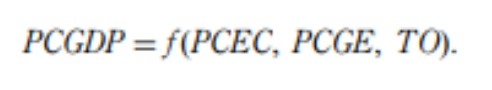
\includegraphics[scale=0.6]{electricity1.jpg}}
    \caption{Formulae 2.1}
\end{figure}
Where PCEC denotes the amount of power consumed per person (in kWh). The PCGDP stands for per capita GDP (constant 2010 in US dollar). PCGE (per capita government final consumption expenditure) and TO (trade of) are both in constant 2010 US dollars. \\
\begin{figure}[htbp]
    \centerline{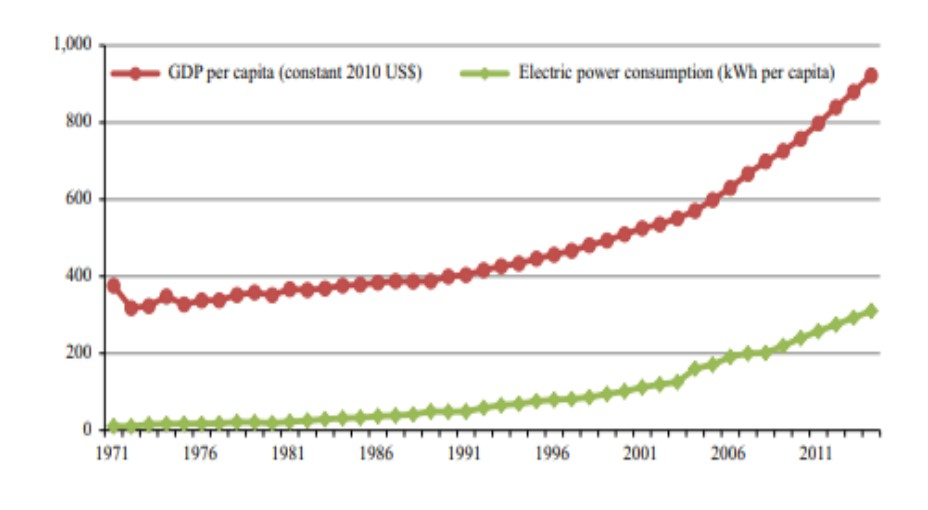
\includegraphics[scale=0.6]{electricity2.jpg}}
    \caption{A plot showing GDP and Electricity consumption}
\end{figure}
Once stationarity or cointegration is established, the econometric version of the aforementioned model linking to GDP and electricity
consumption was delivered as follows: $\alpha$  is the intercept, $\beta$1-$\beta$3 are the coefficients of exogenous variables
and $\varepsilon$  is the error term, all the variables stated in the functional form above are present. \\

\begin{figure}[htbp]
    \centerline{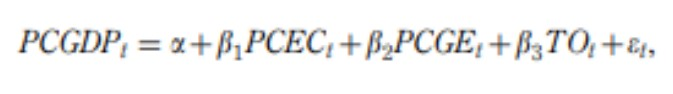
\includegraphics[scale=0.6]{electricity3.jpg}}
    \caption{Formulae 2.2}
\end{figure}
As a result, Strong evidence is being provided by both short-run and long-run coefficients that there is a significant positive relationship between electricity usage.
The bi-directional long-run causation between GDP and electricity consumption is further supported by a combined F-test. The robustness of their long run results was tested using three different estimators.
Their findings of positive electricity consumption-economic for the relationship between the development of financial activities and the economic growth in the country remain robust to all these three estimators .\\
Using this method, their overall study results suggest that the feedback hypothesis, which gives us the census that there is a two-way causal relationship between power consumed and GDP, exists both in the short-run and the long-run, showing that as Bangladesh's economy expands, electricity demand rises and vice versa.
\bigskip
\bigskip
\\
\emph{ D. Can sustainable dvelopment be tracked and measured?}
\\"Sustainable development has broad appeal and little specificity", is a very important quote which summarizes how the paper is present and how it is going to be approached bby the author's of the paper.
The paper tries to address and summarise the facts of what sustainable development means from the perspective of the county and how this can be matched with the growth of the company.
The paper goes tharough and answer "How is sustainable development defined?", "Why characterize and measure sustainable development?", "What and how are goals, indicators, and targets selected?" and  "How are the indicators constructed?"
\\The author also mentions the factors that are to be sustained and what are to be developed in accordance to the summit held on sustainable development that came up with goals. And in
accordance to that we can see that factors as:
\begin{figure}[htbp]
    \centerline{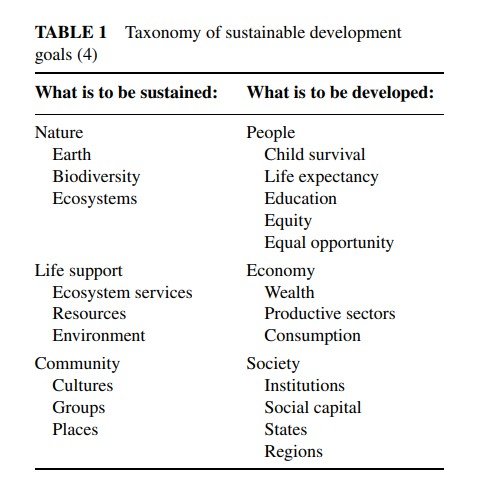
\includegraphics[scale=0.6]{sustainability.jpg}}
    \caption{Figure 3.1}
\end{figure}
\\ The paper concludes by saying that the groundwork of the emergent sustainability science, much work has been done on indicators of
sustainable development and more are to be done on the core topics in this field of sustainability science. This gives the culmination that there is no single indicator that can determine sustainability. And GDP at the end of the day just is a measure for country's growth.
\section{Dataset}
The "Our World in Data" proctors charting of how various different aspects of life impartially put together with GDP of a country. They are an organisation that provides research and data to mark progress against the world's largest problems.
\textbf{Sources:}\\
\begin{itemize}
    \item Our world in data,\textbf{\href{https://ourworldindata.org/}{GDP-electricity and -cereal yield}}
    \item Kaggle,\textbf{\href{https://www.kaggle.com/datasets/programmerrdai/financing-healthcare}{Healthcare financing Dataset}}
\end{itemize}
Since, there exists no one dataset that is feasible for this study a merged datset is need to be produced to calculate the various factors such as production, consumption and expenditure.
Kaggle is an other open-source dataset interceder that helps in finding out clean dataset \emph{(None of which were usable in this case, but it did help identify how such a dataset can be cleaned)}.
The datset that was finally made contained the following:
\begin{center}
    \begin{tabular}{ |c| }
        \hline
        Entity (Country name)       \\
        \hline
        Code                        \\
        \hline
        Year                        \\
        \hline
        Consumption (Electricity)   \\
        \hline
        Production (1.Meat)         \\
        Production (2.Cereal Yield) \\
        \hline
        Expenditure(Healthcare)     \\
        \hline
        GDP                         \\
        \hline
    \end{tabular}
\end{center}
\bigskip
\emph{The Code was the method of accesing a specific country or code together with the year acted as a unique identifier. The GDP is the exploratory variable. There are 2 different values for production due to data discrepancy.}
\section{Initial Insight (EDA)}
In order to understand the nature of the data, some of the attributes that were sorted for and mentioned above were analysed independently and compared on a global and nation-wise scale with 6 different countries for 4 different analysis, in order to find correlations and check inconsistency.
Visualizing such a dataset came up with intersting result which can be seen \textbf{\href{https://github.com/NeerajG03/Economic_Growth-Versus-Factors}{"here"}}.
The first aspect that was observed to see if size of the economy helped us conclude something related to the GDP and this can be seen in the figure shown as such:\\
\begin{figure}[htbp]
    \centerline{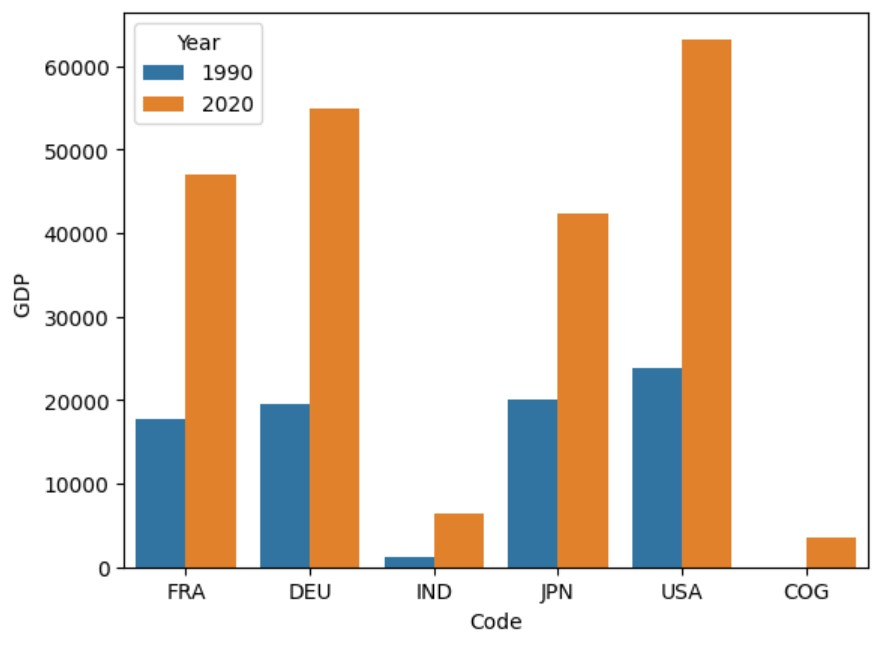
\includegraphics[scale=0.5]{eda1.jpg}}
    \caption{Growth Index}
\end{figure}
\\
The main visualization description that we attained is that meat consumption did not correlate highly with GDP.
This is due to the fact that consumption might vary on a per country basis.
The changes in consumption category of
Hence the change of consumption criteria was made to production of wheat, this still comes up short for many countries that are heavily reliant on meat as their primary source of nutrition.
Another observation from the data was that the correlation of GDP with accordance to healthcare expenditure and electricity consumption were usually high
Finally by Visualizing the finalized dataset seen as such:
\begin{figure}[htbp]
    \centerline{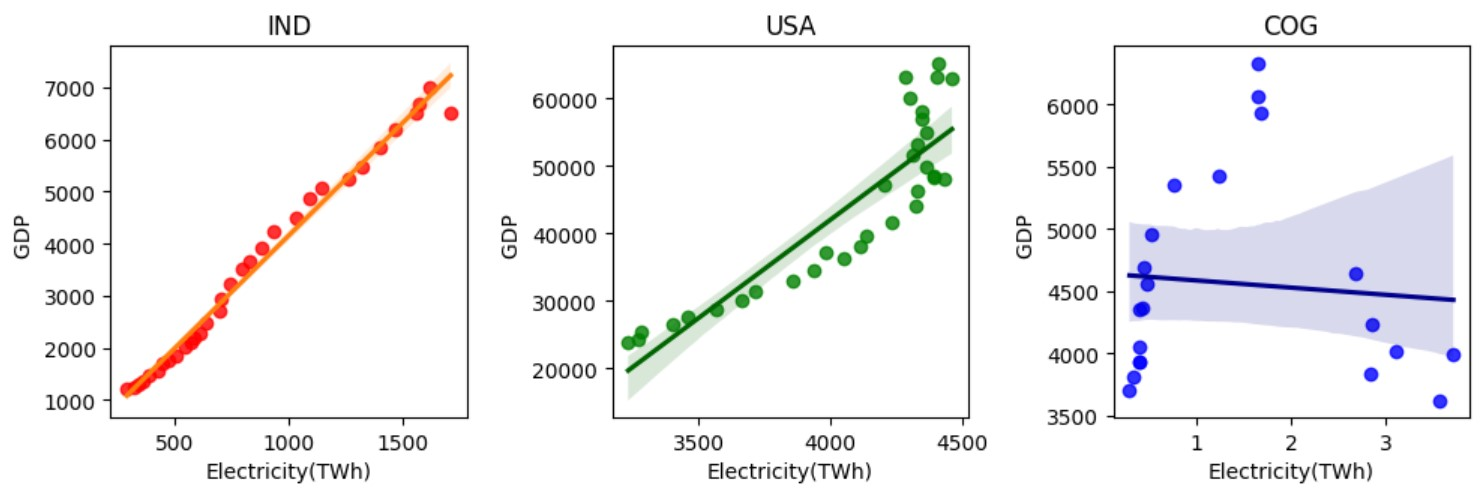
\includegraphics[scale=0.35]{eda2.jpg}}
    \caption{Electricity}
\end{figure}
\begin{figure}[htbp]
    \centerline{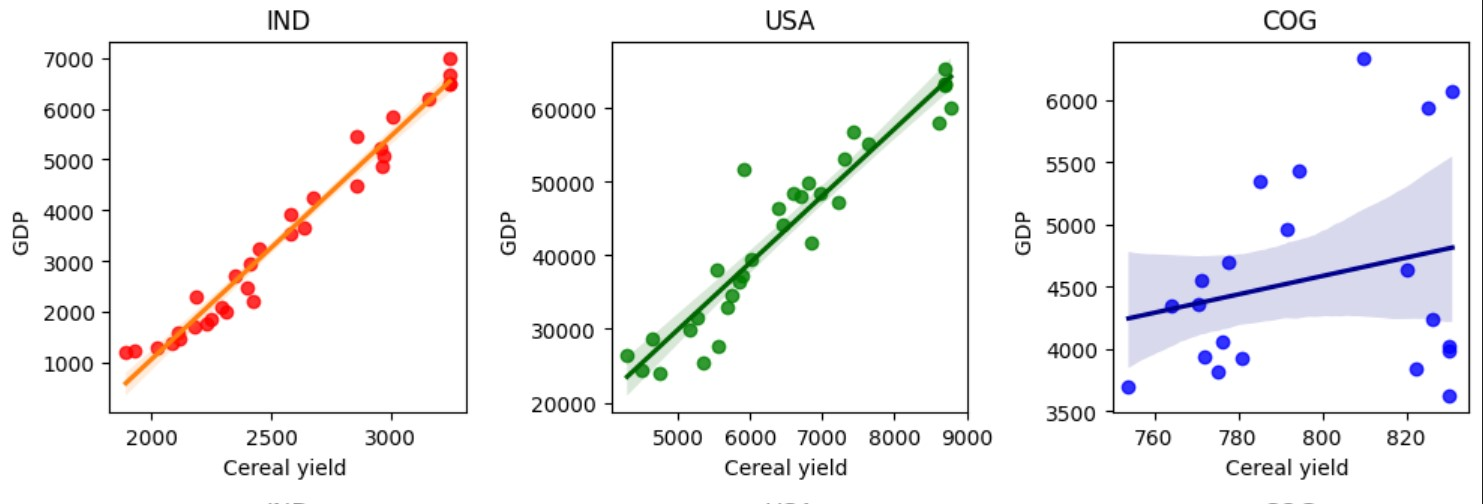
\includegraphics[scale=0.35]{eda3.jpg}}
    \caption{Crop Yield}
\end{figure}
\begin{figure}[htbp]
    \centerline{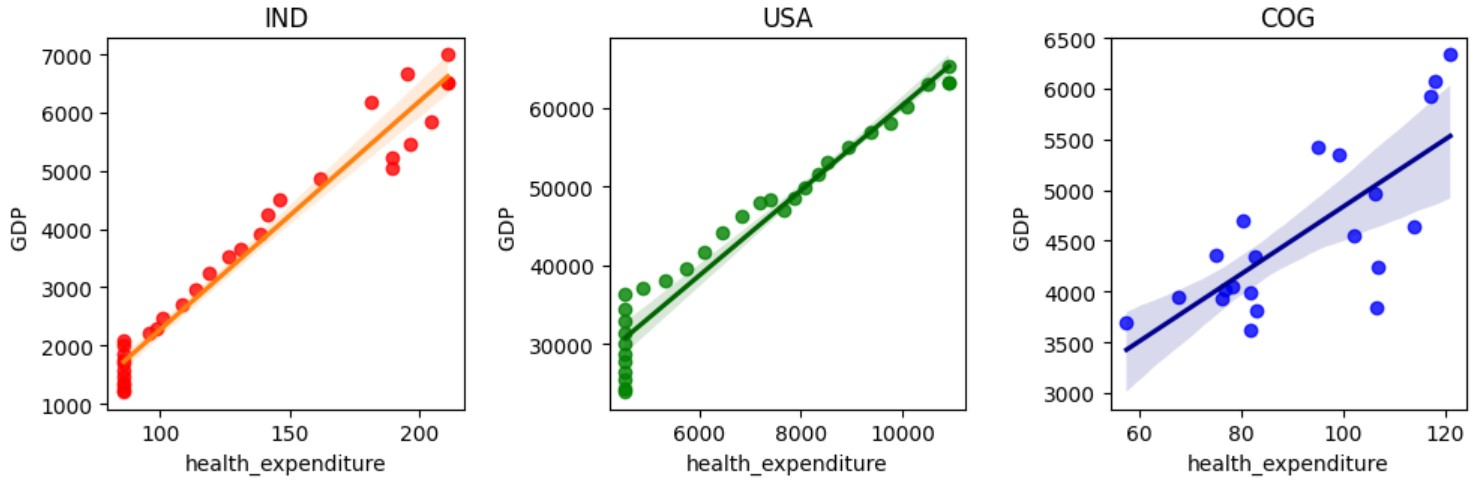
\includegraphics[scale=0.35]{eda4.jpg}}
    \caption{Healthcare Expenditure}
\end{figure}
\emph{(only usually in developing and developed country or countries with stable economy)}. This was especially seen in countries like Congo where the correlation was highly haphazardly correlated with almost all these factors.
\bigskip
\section{Problem Statement and Proposed Solution}
\emph{The WHAT and the WHY?}\\
The meat of the problem is that GDP should be highly correlated to a countrys sustainability development growth rate.
The sustainability development goal is meant to be a problem index that helps to fram a reference for countries that are ahead to fall under a norm to prevent our future from being undesirable.
This not only stands for the developed countries but also for the developing and under-developed countries as these countries need to follow suite and also have a seperately manifested goals as their sustainability goals.\\
This paper tries to predict GDP using the consumption, production and expenditure as factors of influence to see if a country is on track for their macroecnomic development goals.
Our analysis tries to correlate GDP with sustainability development score and see if the countries are on track to meet such goals and also see how long until a ciuntry will meet this criteria, this paper also aims to answer if the measurement of growth of a country is meant to be GDP or if a new way is required to measure sustainablility growth index.
\bigskip\\
\emph{The HOW?}\\
The various methods that this study is going to put forth is the models and visulaization techniques that are used to fullfill the task of the paper's problem statement.
\\For GDP prediction it will be:\\
\begin{itemize}
    \item Linear Regression models
    \item ARIMA Forecasting
    \item Vector Auto Regression
    \item Elastic Net Model
\end{itemize}
For GDP metric evaluation as growth score it will be a simple economic growth versus sustainability score correlation.
And for goal tracking it will be an ARIMA forecasting to check how far a country's economy is from the required SDG(sustainable development goals).

\bigskip
\section{Experimentation and Results}
\subsection{Linear Models}
On the basis of several assumptions, the GDP of the nation was examined. Electricity consumption, healthcare expenditure, and cereal production are taken into account. Over the years of 2017 to 2019, predictions were made concerning GDP growth. The predicted increase/decrease in GDP growth is given in the below table.\\
\begin{figure}[htbp]
    \centerline{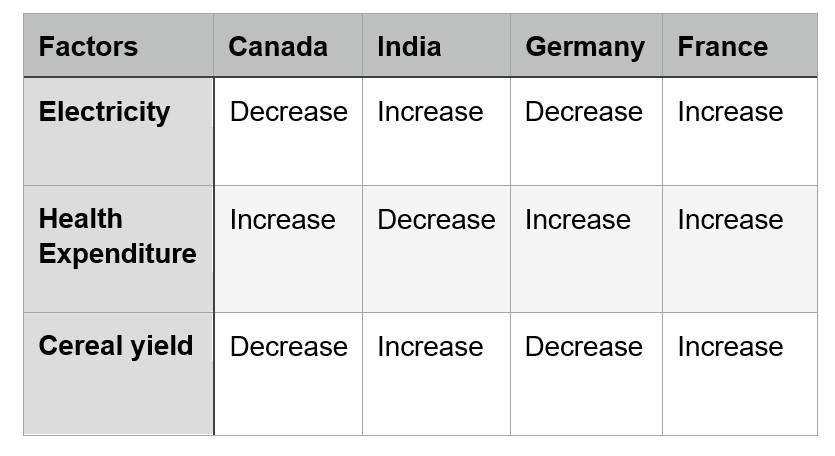
\includegraphics[scale=0.5]{slr.jpg}}
    \caption{SLR Predictions-expected}
\end{figure}
\\
In Canada, the GDP is predicted to be negatively impacted by electricity consumption and cereal output but positively impacted by health spending. India, interestingly, has opposing aspirations. When energy consumption and cereal output are taken into account, India's GDP is predicted to increase favourably; but, if health expenditures are taken into account, the GDP is predicted to decrease.\\
Regarding GDP expansion, Germany and Canada share the same predictions. However, France, which has been significantly impacted positively by the factors mentioned, plans to increase its GDP.
\begin{figure}[htbp]
    \centerline{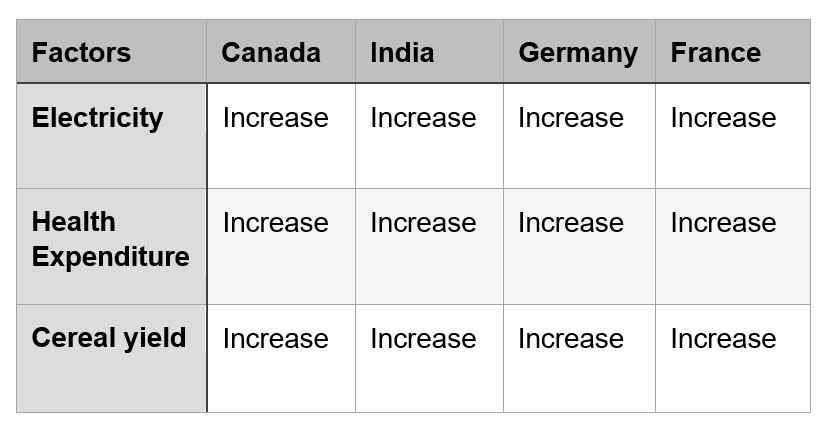
\includegraphics[scale=0.5]{slr2.jpg}}
    \caption{SLR Predictions-observed}
\end{figure}
\\
Surprisingly, the outcome reveals that the three factors—electricity use, health care spending, and cereal production—have a positive influence on all four countries.
\begin{itemize}
    \item Electricity Consumption: India and France consume the most electricity, as was predicted. However, contrary to expectations, GDP grows in Canada and Germany in terms of power consumption. The prevalence of energy- intensive sectors, the high need for heat in cold weather and air conditioning in heat, and other factors could be the reason for this outcome. Hence, affordable electricity combined with high income and purchasing power boost GDP growth.
    \item Health Expenditure: The outcomes for Canada, Germany, and France came out as expected. However, India's GDP growth was positive when compared to health care spending. The reason for this can be related to India's growing population and people's increased attention to their health. The Indian government has launched campaigns and programmes for its people in response to this mindset among the populace, which has led to an increase in GDP.
    \item Cereal Production: India and France's outcome remains as expected. However, when compared to Cereal Production, Canada and Germany — like with electricity use — result in an increase of GDP. The western Canadian provinces of Alberta, Saskatchewan, and Manitoba are perfect for cultivating high-quality, high-protein spring wheat due to their harsh winters and sunny, dry summers. Germany's favourable
          geographic location for cereal production could be one of the variables related to the country's high cereal production and GDP growth.
\end{itemize}
\begin{figure}[htbp]
    \centerline{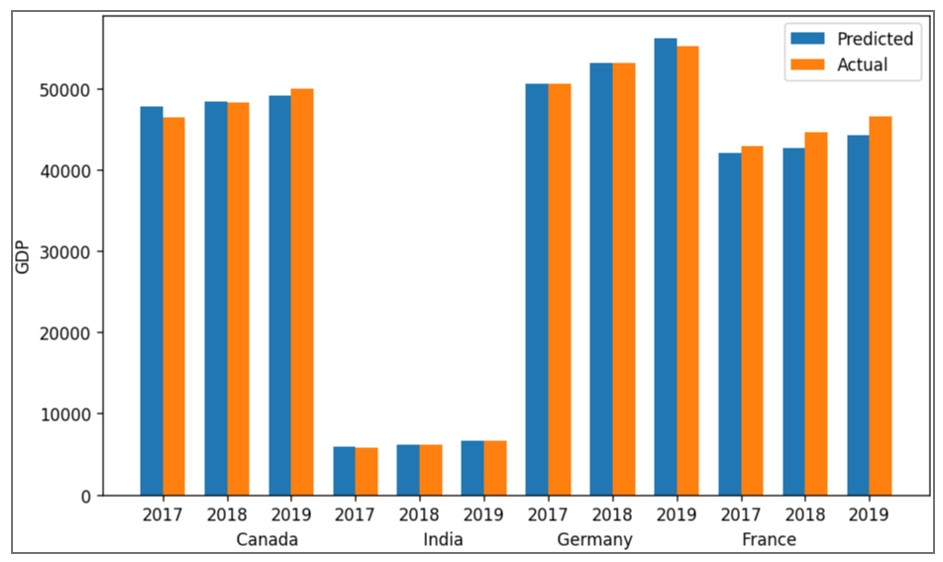
\includegraphics[scale=0.5]{mlr1.jpg}}
    \caption{MLR observation}
\end{figure}
Using MLR, it is anticipated that GDP will have increased between 2017 and 2019 due to a number of factors, including power use, healthcare costs, and cereal output. The three components combined contributions to GDP growth are the clear cause for this prediction. It is reasonable to state that, among the elements taken into account, health expenditures account for the bulk of the GDP contribution in industrialised nations like Canada, Germany, and France. These nations' citizens and governments place a high priority on
public health and have made it mandatory for all citizens to have health insurance, which has contributed to GDP growth.
\\
In contrast, it may be more accurate to say that India's largest source of GDP contribution—its use of electricity—comes from its people.
\\
\emph{Observed}
As expected, the GDP of each of the four nations rises year over year. India has the lowest GDP but is growing, whereas Germany has the highest.

Following are the RMSE of actual and predicted GDP.\\
- Canada: 915.34795\\
- India: 28.46796\\
- Germany: 539.34266\\
- France: 1839.49549\\
It's important to note that the GDP in Germany in 2017 and 2019 was lower than expected. France consistently grows and outperforms GDP projections over the course of three years. India's GDP was roughly stable during the time.
\bigskip
\subsection{ARIMA Modelling}
ARIMA (p, d, q) is a linear model made up of the moving average model MA (q), the autoregressive model AR (p),
and the linear model ARIMA (p, d, q).
Here, p and q may be used to describe the order of the AR model and MA model, respectively.
d is used to represent how many time series differences there are.
\\
Identification of the autoregressive integrated moving average model where the order is
(p,d,q)
Equation 's first step in creating an autoregressive integrated moving average model is
to determine whether the observational time series data are stationary. The series of observations should
be accurately differentiated into a stationary series in order for it to exhibit stationarity.
In order to achieve stationarity, the Auto Correlation Function (ACF) and the
The Partial Auto Correlation Function, or PACF, of the specified time series data sets must be calculated.
The series must be put under suitable differenced order if they are not stationary.
\begin{figure}[htbp]
    \centerline{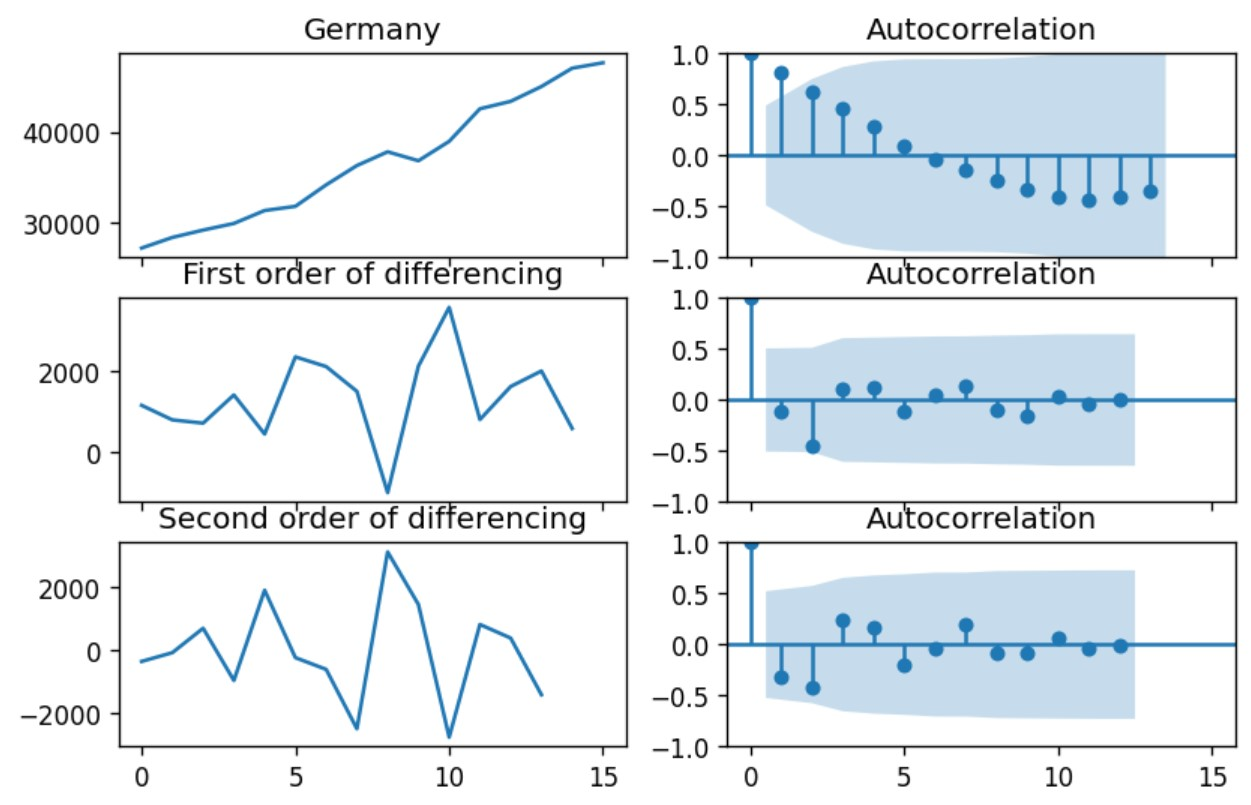
\includegraphics[scale=0.41]{arimaa.jpg}}
    \caption{ARIMA PACF analysis}
\end{figure}

\textbf{Model Identification}\\
Only after transforming the series of observations (sample data) taken into consideration for forecasting into a stationary series, the Autoregressive Integrated Moving Average model is projected. According to the stationary series, there is only a small change in the mean and variance of the observations over time. As shown in Figure (1), it is first determined whether the series of observations from the sample data is stationary or not. It is clear that the series is not stationary. The proper differencing order of the data series under consideration changes non-stationary in mean. It is clear from Figure 2 that the series at the first difference is stationary.
\\
\textbf{ADF Test Chart}
\begin{itemize}
    \item Augmented Dickey-Fuller Statistic: 2.070127 Germany
          \\p-value: 0.998757
    \item Augmented Dickey-Fuller Statistic: 0.209270 India
          \\p-value: 0.97277
\end{itemize}


The ADF (Augemented Dickey Fuller Unit Root Test) is obtained here to demonstrate the stationarity of the series. Clearly, the p-value for the ADF test for the nations of India and Germany is 0.998757 and 0.97277, respectively, which is far higher than the threshold value of 0.05. In order to render the data steady in this situation, we must reject the NULL hypothesis and differentiate the data. Table displays the estimated ADF test results (2). The table suggests that the series of observations is stationary when expressed as a first difference. Therefore, d=1 is used in our ARIMA model (p, d, q).

So now, Finding appropriate values for p and q in the ARIMA model is the current job. The first difference order of the sample data—the correlogram and partial correlogram of the stationary series—is analysed. The sample of data at the first difference is shown in Figure 3 as the autocorrelation function (ACF) and partial autocorrelation function (PACF), respectively.
The q value can be considered as 1, given there is just one lag outside of the threshold area in the ACF plot. The PACF for India is 2 points behind the threshold. But in order to be more conservative, we'll take 1.\\
\begin{figure}[htbp]
    \centerline{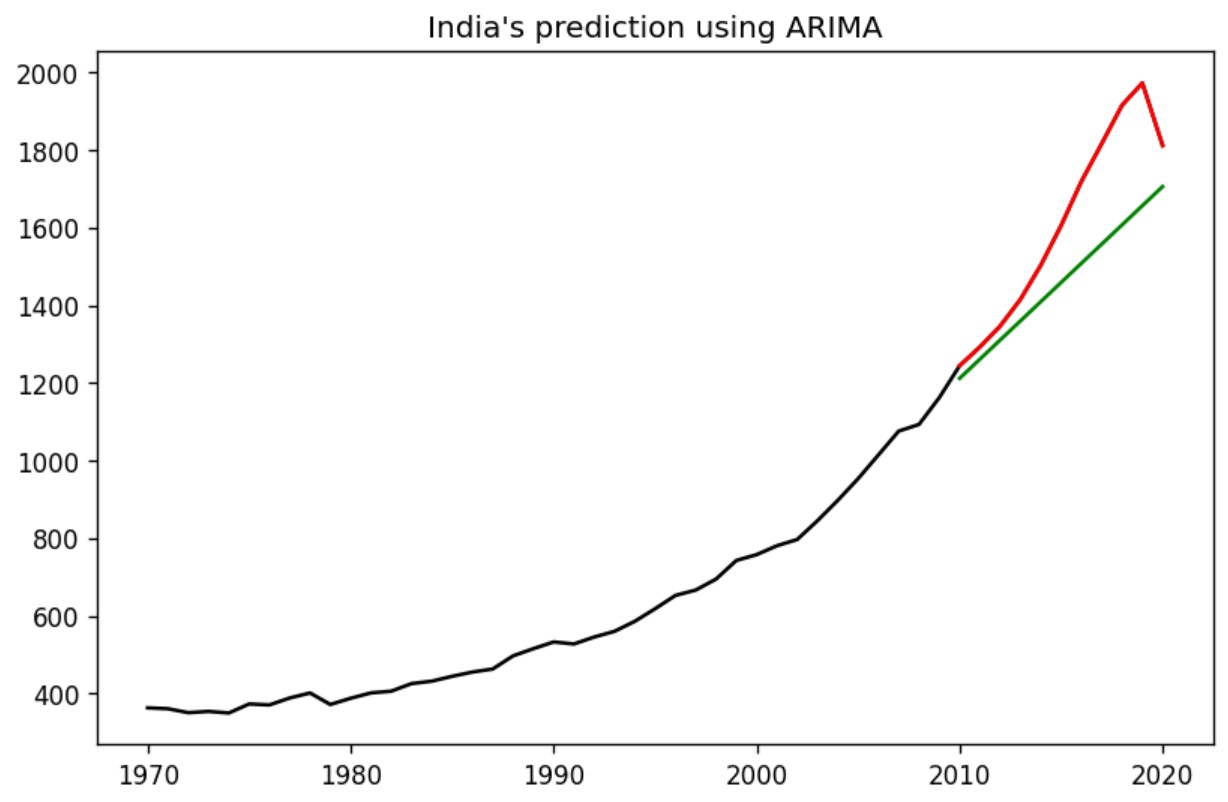
\includegraphics[scale=0.37]{arimaa2.jpg}}
    \caption{ARIMA Forecasting India}
\end{figure}
\\From the observations made from the model we a very low RMSE for higher economies this an be seen by plotting india, germany and china which when done side to side we can see decreasing
value of RMSE the higher the economy is of that country. Although the GDP is influenced by a number of other factors,
the forecasted GDP provided by the Arima model was remarkably accurate.
\bigskip
\subsection{Elastic Net Modelling}
We used elastic net regression to discover a prediction that was superior to the earlier models. Elastic net has the advantage of allowing a balance between the two penalties,
which can lead to better performance on particular problems than a model with just one penalty.
In order to do this, the GDP of Germany and India was anticipated taking into account the variables Electricity(TWh),
Health expenditure, and Cereal yield. These countries were taken to represent 2 stable economies in a cope of larger and smaller value in GDP.
\\
\begin{figure}[htbp]
    \centerline{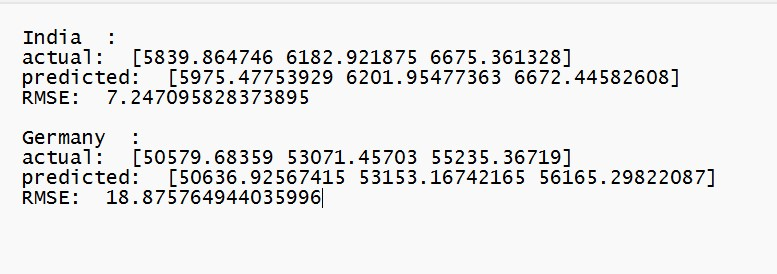
\includegraphics[scale=0.66]{elastic1.jpg}}
    \caption{Elastic Model Observations}
\end{figure}
\\
According to the forecast, the GDPs of Germany and India would both grow by 2019. The actual outcome confirms this,
with RMSE values for India and Germany of 7.25 and 18.75, respectively.
This shows that by penalizing using the L1 and L2 penalty factor we can see a substantially lower GDP across both


\bigskip
\subsection{Sustainability Tracking}
The United Nations Sustainable Development Goals (SDGs) are targets for global development adopted in September 2015, set to be achieved by 2030. All countries of the world have agreed to work towards achieving these goals.\\
\begin{figure}[htbp]
    \centerline{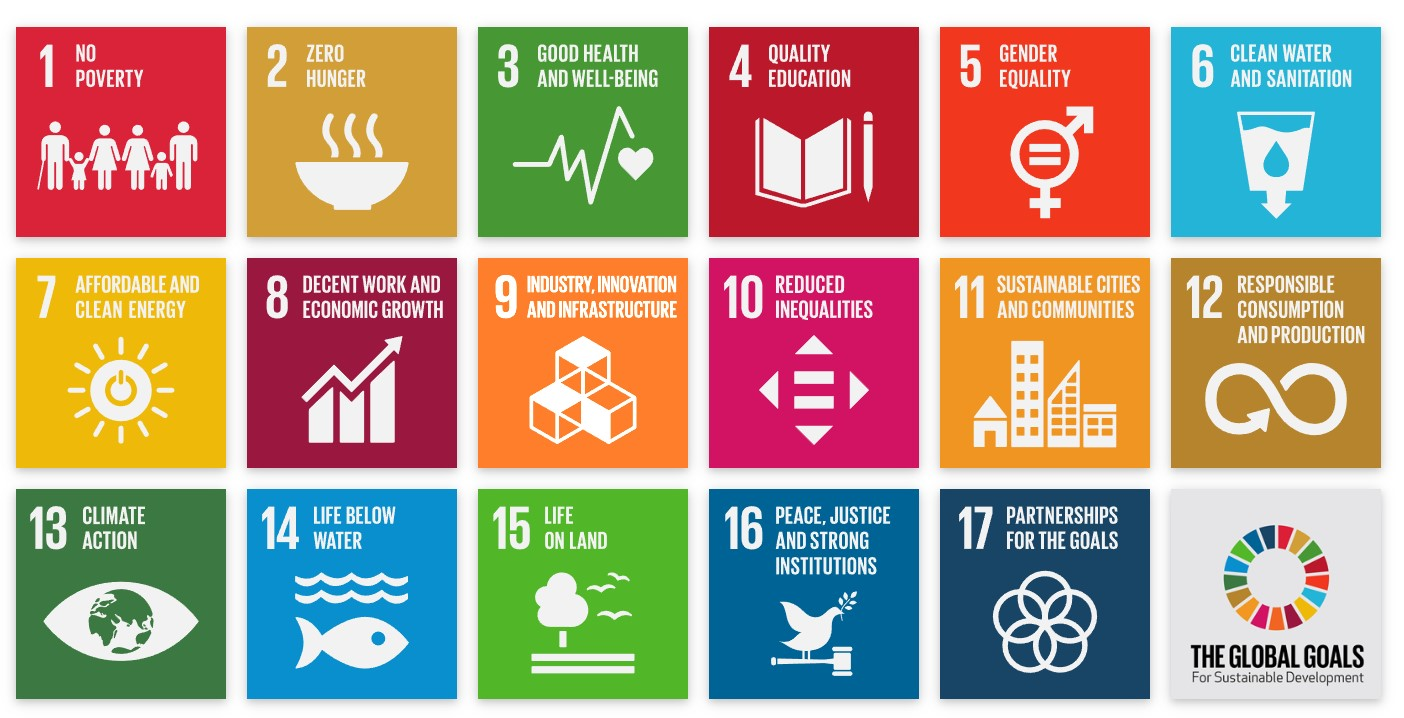
\includegraphics[scale=0.35]{sdg.jpg}}
    \caption{The SDGs}
\end{figure}
\\We can use MA or ARIMA model to see where the sustainability of a acountry is goung and how long it will take for a country to attain such an SDG goal. For many Indicators data is available, but major data gaps remain. If you are aware of high-quality data we have yet to include please notify us. We hope that this collaborative approach allows us to support the United Nations in developing the most complete and up-to-date sources for tracking global progress to 2030.
\bigskip
\section{Conculsion and Inferences}
We have observed that the Elastic net model has the highest accuracy metric when considering the metric to be RMSE for economies that range from low to medium and that the arima model can be used for the economies that are considered in the range of median to high.
This indeed was a very challenging prospect to analyse due to fact of it being a time series data and the sparse availability of said data.
This made us create custom data from scraping, kaggle and our world in data. This also resulted in the project not having a lot of observable units as time kept moving back. Hence
the vector auto regression which is considered to be the best for Multivariate Time Series analysis falls flat rather than be useful in such a circumstance as this.
\\
For the sustainability tracking the model can accurately predict the year a country will reach he goal, this was observed from countries like Ghana and India. This also makes us se the GDP of a country in a new light as
we observe that GDP is no more the appropriate method to see a countrys growth as growth is not just becoming bigger but also about becoming better in multiple-facets of a countrys foot print.
\\\textbf{To summarize}
\begin{itemize}
    \item To predict GDP:
          \begin{itemize}
              \item The elastic net model is considered the best for economies that range from under-developed all the way to developing countries. These can be seen in the example of India and Ghana
              \item The ARIMA model is considered the best when it comes to countries that are considered to be developed or super-nation. This is seen in countries like USA and China.
              \item An exception to the Germany whose GDP can be predicted accurately with both the model.
          \end{itemize}
    \item On the talk of sustainability it is high time that countries look at a better measurement metric to measure growth of a country. This is due to the fact that developing and developed countries need not grow in the traditional sense for their country to prosper.
    \item On the contrary since countries like Ghana do need to grow out of their under-developed state of economy GDP can be seen as a good way to measue growth for such countries.
\end{itemize}
\begin{figure}[htbp]
    \centerline{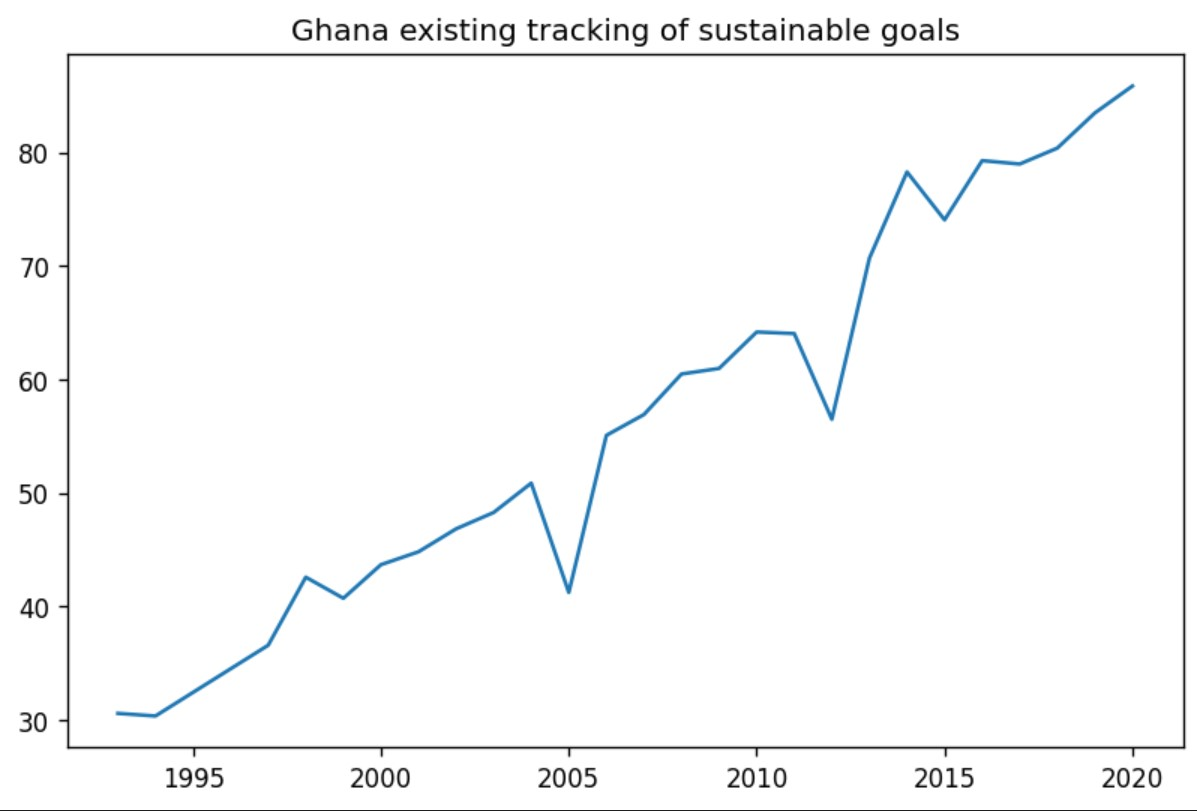
\includegraphics[scale=0.37]{sustainability1.jpg}}
    \caption{Sustainability Tracking vs GDP}
\end{figure}
The figure show that the country can't be tracked using GDP and that we might need a better measure for measuring a growth of a country in the near future that takes into account the ratio between consumption, production, excretion and expenditure.
\bigskip
\section{Acknowledgement}
From the members of this project we would like to extend our gratitude to Dr.Nagegowda who has helped us by providing us the opportunity for being able to create a study on such a topic, and guiding us along the way.
We would like to convey our appreciation towards the CSE department at PES University, for always inspiring us to conduct frequent research and inculcating a problem-solving discipline in us as well.
We would also like to acknowledge our assistant professors and the teaching assistants who have helped in the making and material of the course content and also the teaching assistants who have been constantly providing resources to practice the learnt concepts.
\begin{thebibliography}{00}
    \bibitem{b1} Ahmed Ibne Mahmood, Naznin Hossain, Sojib Bin Zaman,  Shuchita Sharmin Shakeel and Varshil Mehta,  \textbf{\href{https://jmrionline.com/jmri/article/view/72/86}{"An Association of Total Health Expenditure with GDP and Life Expectancy"}}, Vol 1 No 2 (2017) / AU7-AU12.
    \bibitem{b2} Mohammed Tareque and Sima Rani Dey, \textbf{\href{https://www.emerald.com/insight/content/doi/10.1108/JABES-04-2019-0029/full/pdf}{"Electricity consumption and GDP nexus in Bangladesh: a time series investigation"}}
    \bibitem{b3} Global Goals, \textbf{\href{https://www.globalgoals.org/goals/}{"The Global Goals of UN"}} \emph{Now changed from 8 goals to 17 goals}
    \bibitem{b4} Macroeconomics, \textbf{\href{https://www.worldbank.org/en/topic/macroeconomics/overview}{"Macroeconomics at a glance"}}
    \bibitem{b5} Massimiliano Marcellino, \textbf{\href{https://www.researchgate.net/profile/Niels-Haldrup/publication/228650389_A_comparison_of_time_series_models_for_forecasting_GDP_growth_and_inflation/links/0c96051b6b0d0e7951000000/A-comparison-of-time-series-models-for-forecasting-GDP-growth-and-inflation.pdf}{"A comparison of time series models for forecasting GDP growth and inflation"}}, April 2007 Curr. V3
    \bibitem{b5} Thomas M. Parris, Robert W. Kates \textbf{\href{http://www.earthedintl.org/CourseMatls/IEIG/Readings/2b.Characterizing_Measuring_SustDev.pdf}{"A study on factors of sustainability and influence of GDP"}}, July 2003 Curr. V1.0
\end{thebibliography}
\end{document}

